% This is text associated with the open textbook "Open Electromagnetics"
% See immediately below for author, date
% This work is licensed under the Creative Commons Attribution-ShareAlike 4.0 International License. (CC BY-SA 4.0) 
% To view a copy of the license, visit http://creativecommons.org/licenses/by-sa/4.0/

%ORB TITLE Lumped-Element Model
%ORB AUTHOR 0        # S.W. Ellingson, Virginia Tech (ellingson@vt.edu)
%ORB DATE 20180802  # yyyymmdd
%ORB ABSTRACT Lumped-element model of transmission line, leading the telegrapher's equations 

\label{m0029_Lumped-Element_Model} % <-- Must match name of this file and module directory name.  Don't mess with this!
\index{transmission line!lumped-element model|(}
\index{lumped-element model|see{transmission line}}

It is possible to ascertain the relevant behaviors of a transmission line using elementary circuit theory applied to a differential-length lumped-element model of the transmission line.
The concept is illustrated in Figure~\ref{m0029_fTL_to_differential_segments}, which shows a generic transmission line aligned with its length along the $z$ axis.
The transmission line is divided into segments having small but finite length $\Delta z$.
Each segment is modeled as an identical two-port having the equivalent circuit representation shown in Figure~\ref{m0029_fLumpedElementModel}.
The equivalent circuit consists of 4 components as follows:
%
\begin{itemize}
\item  The resistance 
\index{resistance}
$R'\Delta z$ represents the series-combined ohmic resistance of the two conductors.  This should account for {\it both} conductors since the current in the actual transmission line must flow through both conductors.  The prime notation reminds us that $R'$ is resistance \emph{per unit length}; i.e., $\Omega$/m, and it is only after multiplying by length that we get a resistance in $\Omega$. 
\item  The conductance 
\index{conductance}
$G'\Delta z$ represents the leakage of current directly from one conductor to the other.
When $G'\Delta z>0$, the resistance between the conductors is less than infinite, and therefore, current may flow between the conductors.  
This amounts to a loss of power separate from the loss associated with $R'$ above.  $G'$ has units of S/m.  Further note that $G'$ is \emph{not} equal to $1/R'$ as defined above. $G'$ and $R'$ are describing entirely different physical mechanisms (and in principle \emph{either} could be defined as either a resistance or a conductance).
\item  The capacitance 
\index{capacitance}
$C'\Delta z$ represents the capacitance of the transmission line structure.  Capacitance is the tendency to store energy in electric fields and depends on the cross-sectional geometry and the media separating the conductors. $C'$ has units of F/m.
\item The inductance
\index{inductance}
$L'\Delta z$ represents the inductance of the transmission line structure.  Inductance is the tendency to store energy in magnetic fields, and (like capacitance) depends on the cross-sectional geometry and the media separating the conductors.
$L'$ has units of H/m.
\end{itemize}  
%
\begin{figure}
\begin{center}
\pdftooltip{{  % note double braces
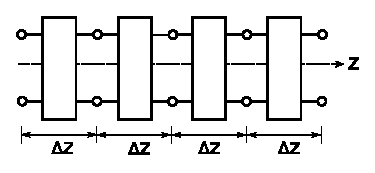
\includegraphics[width=2.5in]{modules/m0029_fTL_to_differential_segments.eps}
}}{Four rectangles arranged in a horizontal line intersected in the middle by a dashed arrow pointing to the right labeled z. The 2 nodes of each rectangle are shown joining the next rectangle to the right. The distance from node to node horizontally is Delta z.}
\end{center} 
\caption{\label{m0029_fTL_to_differential_segments}
Interpretation of a transmission line as a cascade of discrete series-connected two-ports.}
\end{figure}
%
\begin{figure}
\begin{center}
\pdftooltip{{  % note double braces
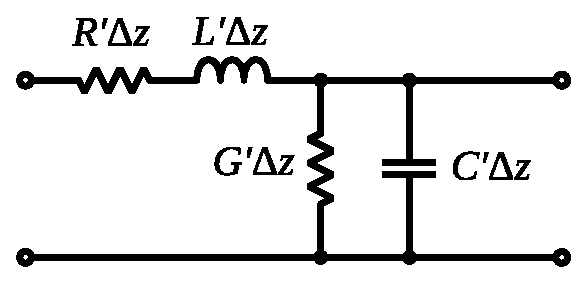
\includegraphics[width=2in]{modules/m0029_Transmission_line_element_se170804.eps}
}}{From left to right, a resistor and inductor in series then connected to a resistor and capacitor in parallel. The left (series) resistor is labeled R' Delta z. 
The inductor is labeled L' Delta z. On the left vertical line, a resistor symbol represents G’ Delta z. On the right vertical line, a capacitor symbol represents C Delta z.}
\end{center} 
%\vspace{2in}
% https://commons.wikimedia.org/wiki/File:Transmission_line_element.svg
\centerline{\scriptsize 
\copyright~\hyperref[m0029_fLumpedElementModel_Credit]{Omegatron} 
\href{https://creativecommons.org/licenses/by-sa/3.0/deed.en}{CC BY~SA 3.0 Unported} (modified) 
} 
\caption{
\label{m0029_fLumpedElementModel}
Lumped-element equivalent circuit model for each of the two-ports in Figure~\ref{m0029_fTL_to_differential_segments}.
}
\end{figure}

In order to use the model, one must have values for $R'$, $G'$, $C'$, and $L'$.   
Methods for computing these parameters are addressed elsewhere in this book. 

\index{transmission line!lumped-element model|)}

